\documentclass[journal,12pt,twocolumn]{IEEEtran}

\usepackage{setspace}
\usepackage{gensymb}

\singlespacing


\usepackage[cmex10]{amsmath}

\usepackage{amsthm}

\usepackage{mathrsfs}
\usepackage{txfonts}
\usepackage{stfloats}
\usepackage{bm}
\usepackage{cite}
\usepackage{cases}
\usepackage{subfig}
 
\usepackage{longtable}
\usepackage{multirow}

\usepackage{enumitem}
\usepackage{mathtools}
\usepackage{steinmetz}
\usepackage{tikz}
\usepackage{circuitikz}
\usepackage{verbatim}
\usepackage{tfrupee}
\usepackage[breaklinks=true]{hyperref}
\usepackage{graphicx}
\usepackage{tkz-euclide}
\usepackage{amsmath}

\usetikzlibrary{calc,math}
\usepackage{listings}
    \usepackage{color}                                            %%
    \usepackage{array}                                            %%
    \usepackage{longtable}                                        %%
    \usepackage{calc}                                             %%
    \usepackage{multirow}                                         %%
    \usepackage{hhline}                                           %%
    \usepackage{ifthen}                                           %%
    \usepackage{lscape}     
\usepackage{multicol}
\usepackage{chngcntr}

\DeclareMathOperator*{\Res}{Res}

\renewcommand\thesection{\arabic{section}}
\renewcommand\thesubsection{\thesection.\arabic{subsection}}
\renewcommand\thesubsubsection{\thesubsection.\arabic{subsubsection}}

\renewcommand\thesectiondis{\arabic{section}}
\renewcommand\thesubsectiondis{\thesectiondis.\arabic{subsection}}
\renewcommand\thesubsubsectiondis{\thesubsectiondis.\arabic{subsubsection}}



\def\inputGnumericTable{}                                 %%

\lstset{
%language=C,
frame=single, 
breaklines=true,
columns=fullflexible
}
\begin{document}


\newtheorem{theorem}{Theorem}[section]
\newtheorem{problem}{Problem}
\newtheorem{proposition}{Proposition}[section]
\newtheorem{lemma}{Lemma}[section]
\newtheorem{corollary}[theorem]{Corollary}
\newtheorem{example}{Example}[section]
\newtheorem{definition}[problem]{Definition}

\newcommand{\BEQA}{\begin{eqnarray}}
\newcommand{\EEQA}{\end{eqnarray}}
\newcommand{\define}{\stackrel{\triangle}{=}}
\bibliographystyle{IEEEtran}
\providecommand{\mbf}{\mathbf}
\providecommand{\pr}[1]{\ensuremath{\Pr\left(#1\right)}}
\providecommand{\qfunc}[1]{\ensuremath{Q\left(#1\right)}}
\providecommand{\sbrak}[1]{\ensuremath{{}\left[#1\right]}}
\providecommand{\lsbrak}[1]{\ensuremath{{}\left[#1\right.}}
\providecommand{\rsbrak}[1]{\ensuremath{{}\left.#1\right]}}
\providecommand{\brak}[1]{\ensuremath{\left(#1\right)}}
\providecommand{\lbrak}[1]{\ensuremath{\left(#1\right.}}
\providecommand{\rbrak}[1]{\ensuremath{\left.#1\right)}}
\providecommand{\cbrak}[1]{\ensuremath{\left\{#1\right\}}}
\providecommand{\lcbrak}[1]{\ensuremath{\left\{#1\right.}}
\providecommand{\rcbrak}[1]{\ensuremath{\left.#1\right\}}}
\theoremstyle{remark}
\newtheorem{rem}{Remark}
\newcommand{\sgn}{\mathop{\mathrm{sgn}}}
\providecommand{\abs}[1]{\l\vert#1\r\vert}
\providecommand{\res}[1]{\Res\displaylimits_{#1}} 
\providecommand{\norm}[1]{\lVert#1\rVert}
%\providecommand{\norm}[1]{\lVert#1\rVert}
\providecommand{\mtx}[1]{\mathbf{#1}}
\providecommand{\mean}[1]{E\l[ #1 \r]}
\providecommand{\fourier}{\overset{\mathcal{F}}{ \rightleftharpoons}}
%\providecommand{\hilbert}{\overset{\mathcal{H}}{ \rightleftharpoons}}
\providecommand{\system}{\overset{\mathcal{H}}{ \longleftrightarrow}}
	%\newcommand{\solution}[2]{\textbf{Solution:}{#1}}
\newcommand{\solution}{\noindent \textbf{Solution: }}
\newcommand{\cosec}{\,\text{cosec}\,}
\providecommand{\dec}[2]{\ensuremath{\overset{#1}{\underset{#2}{\gtrless}}}}
\newcommand{\myvec}[1]{\ensuremath{\begin{pmatrix}#1\end{pmatrix}}}
\newcommand{\mydet}[1]{\ensuremath{\begin{vmatrix}#1\end{vmatrix}}}
\numberwithin{equation}{subsection}
\makeatletter
\@addtoreset{figure}{problem}
\makeatother
\let\StandardTheFigure\thefigure
\let\vec\mathbf
\renewcommand{\thefigure}{\theproblem}
\def\putbox#1#2#3{\makebox[0in][l]{\makebox[#1][l]{}\raisebox{\baselineskip}[0in][0in]{\raisebox{#2}[0in][0in]{#3}}}}
     \def\rightbox#1{\makebox[0in][r]{#1}}
     \def\centbox#1{\makebox[0in]{#1}}
     \def\topbox#1{\raisebox{-\baselineskip}[0in][0in]{#1}}
     \def\midbox#1{\raisebox{-0.5\baselineskip}[0in][0in]{#1}}
\vspace{3cm}
\title{Assignment 4}
\author{Mirha Sidheek}
\maketitle
\newpage
\bigskip
\renewcommand{\thefigure}{\theenumi}
\renewcommand{\thetable}{\theenumi}
Download all python codes from 
\begin{lstlisting}
https://github.com/mirhasidheek7213/InternshipIITH/tree/main/Assignment-4/Codes
\end{lstlisting}

%
and latex-tikz codes from 
%
\begin{lstlisting}
https://github.com/mirhasidheek7213/InternshipIITH/blob/main/Assignment-4/Assignment4.tex
\end{lstlisting}

\section{\textbf{Question No. 2.6 - Vectors}}

 Are the points $\vec{A} = \myvec{3\\6\\9}$ , $\vec{B} = \myvec{10\\20\\30}$, $\vec{C} = \myvec{25\\-41\\5}$, 
the vertices of a right angled triangle?
 
%

\section{\textbf {Solution}}
Given, 

\begin{align}
   \vec{A} = \myvec{3\\6\\9} , \vec{B} = \myvec{10\\20\\30}, \vec{C} = \myvec{25\\-41\\5} 
\end{align}

To check if the vertices are of a right angled triangle we have to prove $(\vec{B}-\vec{A})^\top(\vec{C}-\vec{A})=0$, $(\vec{A}-\vec{B})^\top(\vec{C}-\vec{B})=0$ ,$(\vec{A}-\vec{C})^\top(\vec{B}-\vec{C})=0$, If the triangle is right angled at A, B and C respectively
\\
\\
\subsection{Checking if $\angle A ={90}\degree$}
We have to prove,
\begin{align}
   (\vec{B}-\vec{A})^\top(\vec{C}-\vec{A})=0
\end{align}

\begin{align}
    \vec B - \vec A = \myvec{7\\14\\21}
\end{align}

\begin{align}
     \vec C - \vec A = \myvec{22\\-47\\-4}
\end{align}
Now,
\begin{align}
     (\vec{B}-\vec{A})^\top(\vec{C}-\vec{A})=\myvec{7\ 14\ 21}\myvec{22\\-47\\-4}
\end{align}

\begin{align}
\implies 154-658-17 = -521
\end{align}
 Hence,  $(\vec{B}-\vec{A})^\top(\vec{C}-\vec{A})\neq 0$. Therefore the triangle is not right angled at A.

\subsection{Checking if $\angle B ={90}\degree$}
We have to prove,
\begin{align}
   (\vec{A}-\vec{B})^\top(\vec{C}-\vec{B})=0
\end{align}

\begin{align}
    \vec A - \vec B = \myvec{-7\\-14\\-21}
\end{align}

\begin{align}
     \vec C - \vec B = \myvec{15\\-61\\-25}
\end{align}
Now,
\begin{align}
     (\vec{A}-\vec{B})^\top(\vec{C}-\vec{B})=\myvec{-7\ -14\ -21}\myvec{15\\-61\\-25}
\end{align}

\begin{align}
\implies -105+854+525 = 1274
\end{align}
 Hence,  $(\vec{A}-\vec{B})^\top(\vec{C}-\vec{B})\neq 0$. Therefore the triangle is not right angled at B.

\subsection{Checking if $\angle C ={90}\degree$}
We have to prove,
\begin{align}
   (\vec{A}-\vec{C})^\top(\vec{B}-\vec{C})=0
\end{align}

\begin{align}
    \vec A - \vec C = \myvec{-22\\47\\4}
\end{align}

\begin{align}
     \vec B - \vec C = \myvec{-15\\61\\25}
\end{align}
Now,
\begin{align}
     (\vec{A}-\vec{C})^\top(\vec{B}-\vec{C})=\myvec{-22\ 47 \ 4}\myvec{-15\\61\\25}
\end{align}

\begin{align}
\implies 330+2867+200 = 3397
\end{align}
 Hence,  $(\vec{A}-\vec{C})^\top(\vec{B}-\vec{C})\neq 0$. Therefore the triangle is not right angled at B.
\\
Since these vertices do not form right angles,they are not vertices of a right angled triangle
\begin{figure}[!h]
         \centering
         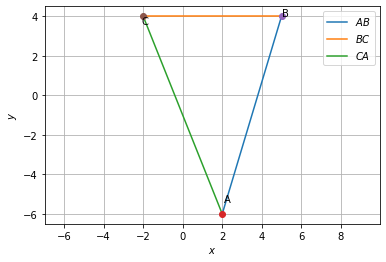
\includegraphics[width=\columnwidth]{Figure.png}
         \caption{Plot of the triangle}
         \label{Figure}
\end{figure}
\end{document}